\documentclass[11pt, oneside]{article}   	% use "amsart" instead of "article" for AMSLaTeX format
\usepackage{hl_short}
\usepackage{geometry}                		% See geom\dagetry.pdf to learn the layout options. There are lots.
\geometry{a4paper}                   		% ... or a4paper or a5paper or ... 
%\geometry{landscape}                		% Activate for for rotated page geometry
%\usepackage[parfill]{parskip}    		% Activate to begin paragraphs with an empty line rather than an indent
\usepackage{graphicx}				% Use pdf, png, jpg, or eps§ with pdflatex; use eps in DVI mode
\usepackage{array}							% TeX will automatically convert eps --> pdf in pdflatex		
\usepackage{amssymb,amsmath}
\usepackage{cite}
\usepackage[final]{fixme}
\usepackage{pdfpages}
\usepackage{tabularx}
\usepackage{fancyheadings}
\usepackage{lastpage}
\usepackage{tikz}
\usetikzlibrary{shapes,arrows}
\usepackage{float}
\usepackage{hyperref}
\usepackage{url}

\newcommand{\comp}[1]{{\sf #1}}

\parskip 6pt % 1pt = 0.351 mm
\parindent 0pt

\pagestyle{fancy}
\lhead{\tiny FP7-ICT 619209 / AMIDST}
\chead{\tiny Page {\thepage} of \pageref{LastPage} \\}
\rhead{\tiny Public}
\renewcommand{\footrulewidth}{0.4pt}
\cfoot{}

\newcommand{\drop}[1]{}

\numberwithin{figure}{section}
\numberwithin{equation}{section}
\numberwithin{table}{section}

\usepackage{pdfpages}

\begin{document}

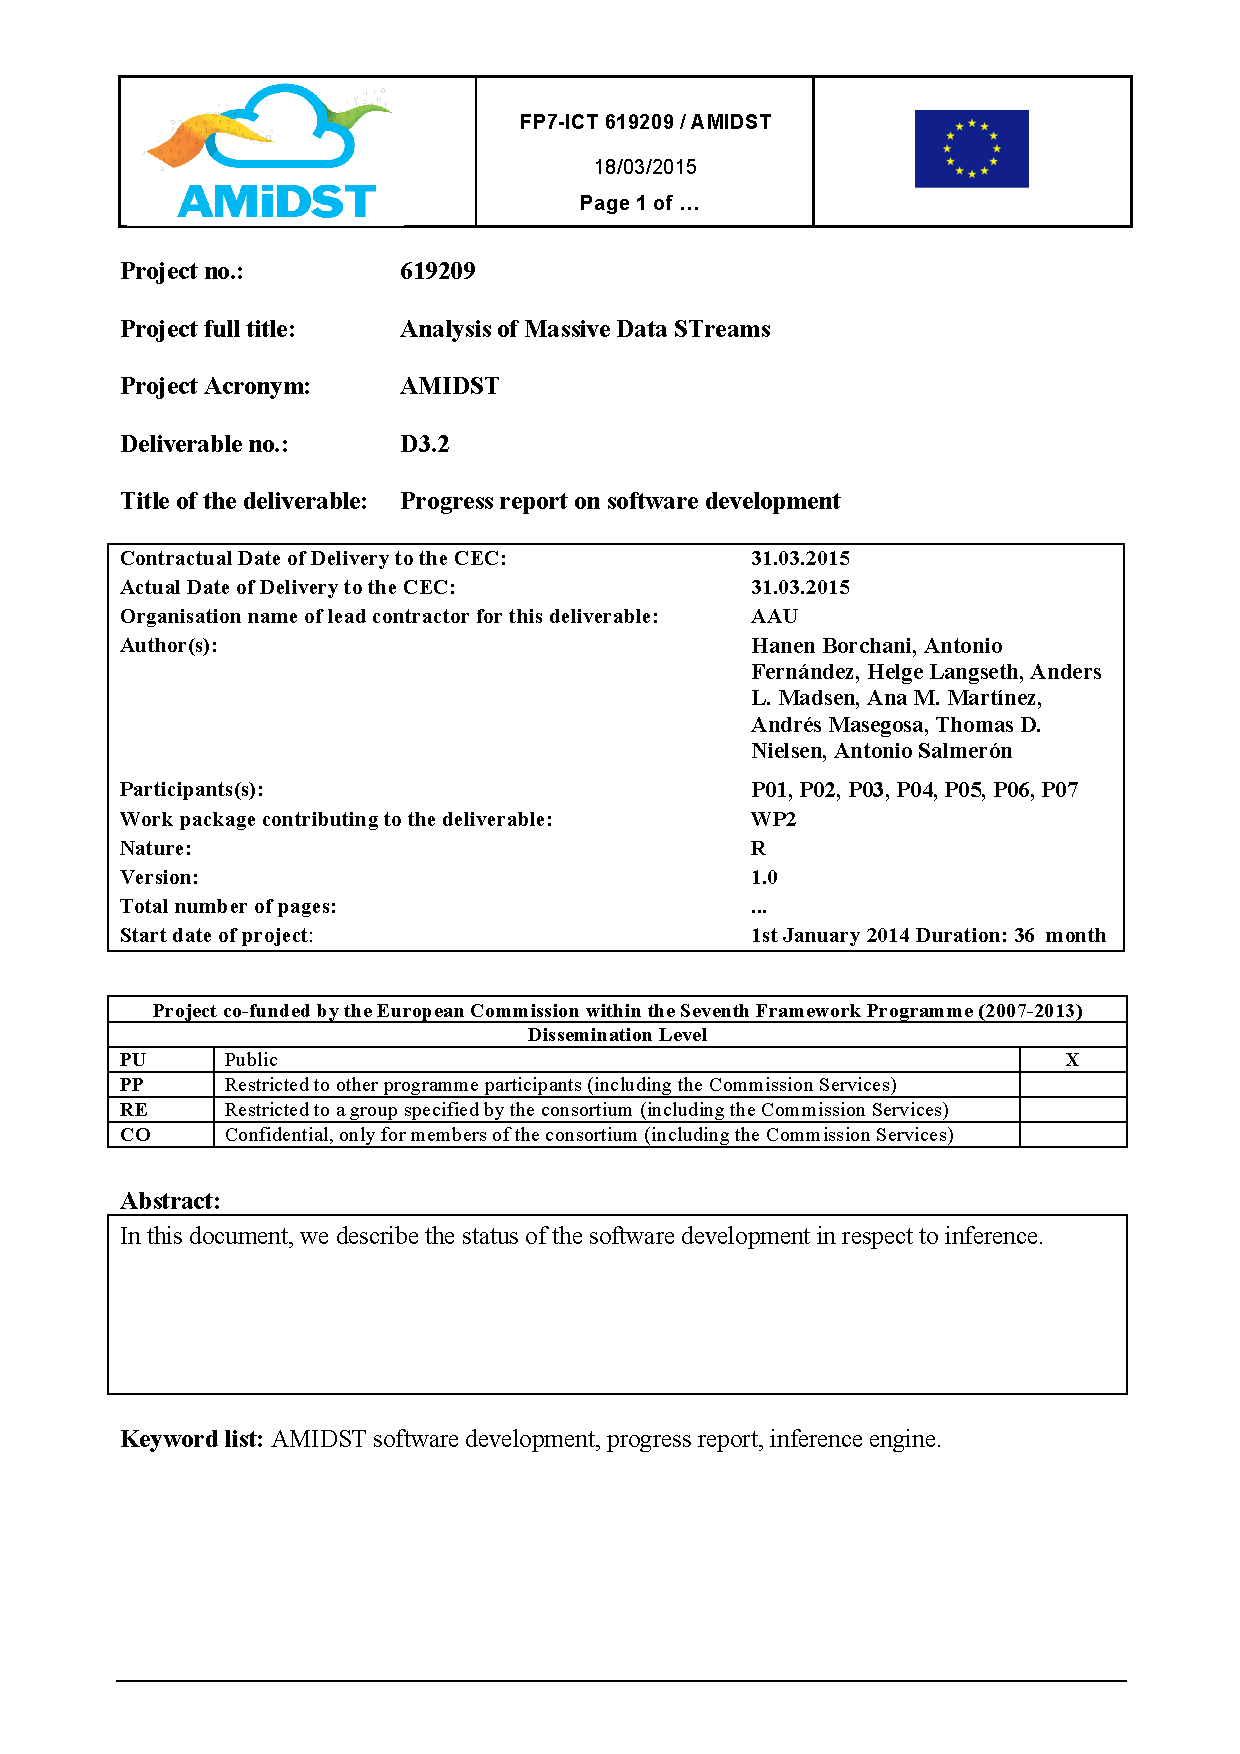
\includepdf[pages={1}]{figures/FrontPage.pdf}

%-------------------------- Table of contents --------------------------
\tableofcontents

\newpage

%-------------------------- Document History --------------------------
\section*{Document history}

\begin{table}[htbp]
  \centering
  \begin{tabularx}{\linewidth}{|p{13mm}| p{18mm}| X | X |} \hline
    {\bf Version} & {\bf Date} & {\bf Author (Unit)} & {\bf Description} \\ \hline
    v0.3 & 16/03/2015~ & All consortium members & The software library implementation for the AMIDST modelling framework discussed and established \\ \hline
    v0.6 & 24/03/2015~ & Hanen Borchani, Antonio Fern\'andez, Ana M. Mart\'inez, Andr\'es Masegosa & Initial version of document finished and reviewed  \\ \hline
    v1.0 & 31/03/2015~ & Hanen Borchani, Antonio Fern\'andez, Helge Langseth, Anders L. Madsen, Ana M. Mart\'inez, Andr\'es Masegosa, Thomas D. Nielsen, Antonio Salmer\'on & Final version of document  \\ \hline
  \end{tabularx}
\end{table}

\newpage

%----------------------------------------------------------------------------
%--------------------------------------------------------------------------------------------------
\section{Executive summary}\label{section:executiveSummary}
%--------------------------------------------------------------------------------------------------

% Consider the diagrams from D4.1
% Extend the functionalities 
% Focus more on inference because it is related to WP3
% Write an introduction to inference (check D3.1, restructure, VMP)
% more details on implemented algorithms
% Description of the implementation with example of use
%----------------------------------------------------------------------------

\newpage

%----------------------------------------------------------------------------
\section{Introduction}

Even though the number of algorithms designed for learning on streaming data is increasing, there is still not a unified and well accepted way for evaluating them.  This is because testing and evaluating algorithms that are designed to work on streaming data are more difficult those designed to work on static data.  There are both statistical and computational reasons for this.  

Static data is data, where each instance can be assumed to be identically and independently distributed i.i.d.  On streaming data, one can often not assume that data instances are i.i.d.  Moreover, the algorithms are often designed to weight measurements that are close to the actual time step higher than measurements that are further back.  On streaming data, we must therefore assume that data are generated from underlying distributions that are time dependent and also that the algorithms themselves are time dependent.  

Computational challenges are related to the fact that the data come from an open-ended data stream, conceptually infinitely long, which imposes practical challenges related to restrictions on cpu-time and memory allocation.  

Various error measures related to stream data has been proposed in the papers of Gama et. al. \cite{Gam09}, \cite{Gam09_2}, \cite{Gam12}.  A loss function is typically related to the penalty of misclassifications on classification problems or residuals in regression models.  The holdout error is basically the average loss on a holdout dataset of fixed size.  The predictive sequential, or \emph{prequential} error is defined as the average loss function up to time step $i$, where $i$ is the current time step.  Moreover, it was also suggested to use a prequental error measure, which involved a forgetting factor such as using a time window or fading factors.  In paper \cite{Gam12}, convergence towards the Bayes error was shown for all these performance measures provided that the learners are consistent and data are i.i.d.  Moreover, it was shown that if data was allowed to drift over time, meaning that samples are only locally i.i.d, then the prequental error measures with forgetting mechanisms were favourable.

\todo{Relate to other work on streaming data as well.}

The applications that are covered in this report have different characteristics than the applications discussed in \cite{Gam12}.  Some problem will be evaluated on a holdout dataset assuming i.i.d and a stationary algorithm.  Other problems can not assume i.i.d on a local scale, but stationarity can be assumed on a larger time scale.  

In this paper we will establish formal procedures for testing and evaluating the developed models and algorithms. This includes specification what metrics are relevant to use to quantify the ability of the AMIDST system, such as relevant formalization of loss functions, maximum response-times, memory limits and output format.  The paper will also include 
considerations about what quantitative improvements AMIDST should obtain over state of the art.

In section \ref{sec:methodology}, AMIDST relevant methodologies for evaluation of both batch and streaming algorithms are identified and discussed.  This section forms the foundation of the subsequent sections, where the exact evaluation routines for each use case provider is given. These sections contains a description of the requirements related to evaluation as described in Delivery 1.2, a short description of the algorithms and the data and finally methods for evaluating predictive and runtime performances.  Section \ref{sec:conclusion} concludes the report.


%\quote{\emph{Task description: In this task we will establish formal procedures for testing and evaluating the
%    developed models and algorithms. This includes specification of maximum response-times, output format,
%    relevant formalization of loss functions, investigations into what metrics are relevant to use to quantify
%    the ability of the AMIDST system, and considerations about what quantitative improvements AMIDST should
%    obtain over state of the art.}}
%
%
%From Helge's slides at the WP 3 kickoff meeting:
%\begin{itemize}
%\item Massive datasets: find relevant techniques, ensure scalability, etc.
%\item Online evaluation of streams: find relevant techniques, ensure scalability, define behavior in changing environment, etc.
%\item Significance of results, e.g., considering changing environment vs. ``reproducability'', distribution for test-statistic, significance levels/sizes of test-sets, etc.
%\end{itemize}

%----------------------------------------------------------------------------

%----------------------------------------------------------------------------
\section{Preliminaries}\label{Section:Preliminaries}

%BN, OOBN, Dynamic BN.
%Preliminaries for the temporal series data analysis: correlograms, partial correlograms. %Preliminaries for the AMIDST models.
%----------------------------------------------------------------------------

%----------------------------------------------------------------------------
%------------------------------------------------------------------------------------------------------------
\section{Inference engine} \label{sec:InferenceEngine}
%------------------------------------------------------------------------------------------------------------

In this section we provide an overview of the current implementation status of the AMIDST toolbox related to inference algorithms. Figure \ref{Figure:InferenceEngine} illustrates the main core components of the toolbox. The color coding in the figure summarizes the implementation status: blue boxes represent software components that have been implemented in the AMIDST toolbox and green boxes represent components that are part of the software design specification but which have not yet been implemented.

\begin{figure}[ht!]
\begin{center}
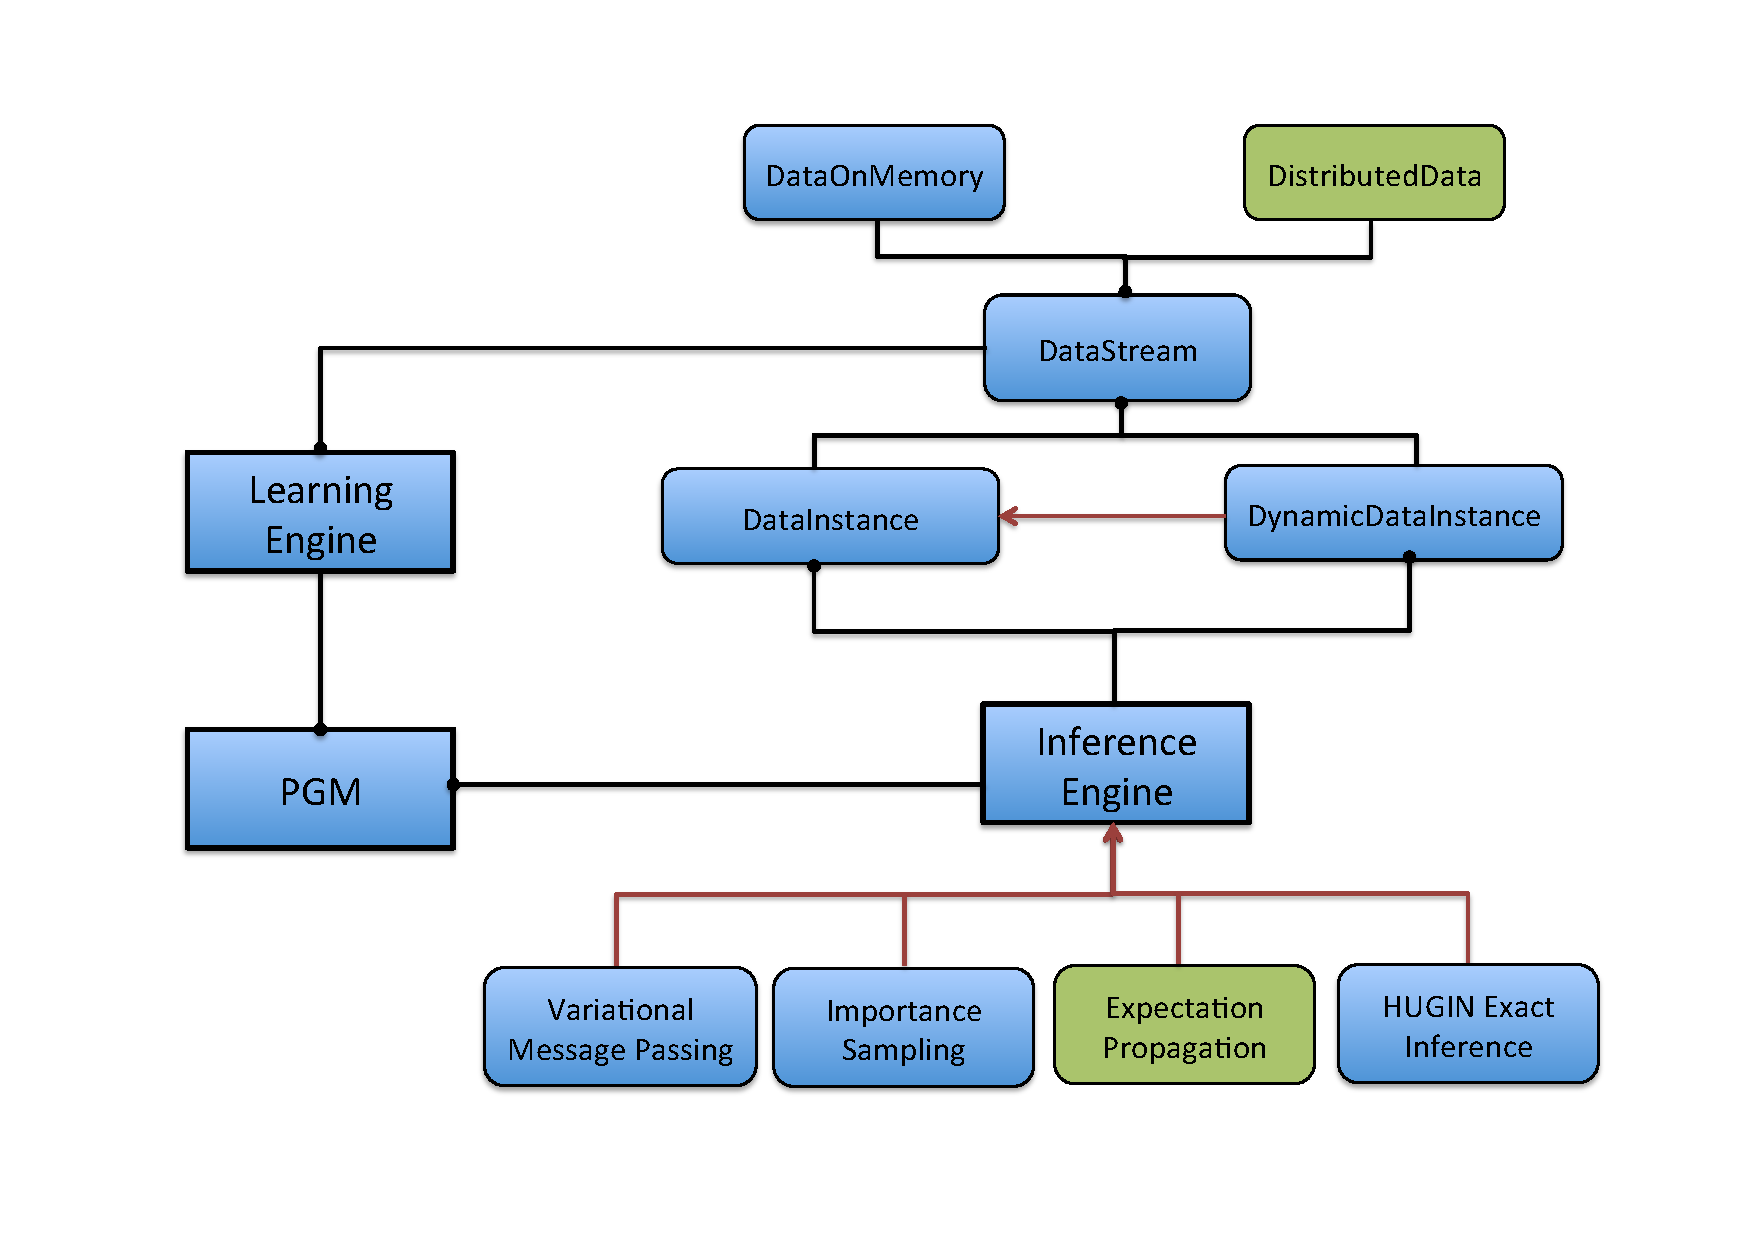
\includegraphics[width=\linewidth]{./figures/InferenceEngine}
\vspace{-0.5in}
\caption{\label{Figure:InferenceEngine} Illustration of AMIDST toolbox main core components. Nomenclature: The boxes in the
      figure represent software components (sets, possibly singletons, of classes), a rounded-arc going from $X$ to $Y$ indicates that $Y$ 'uses/references' $X$, and an arc with an arrow from $X$ to $Y$ implies inheritance.}
\end{center}
\end{figure}

Note that some of the core components of the AMIDST toolbox, shown in Figure \ref{Figure:InferenceEngine}, have already been introduced in the previous deliverables. Deliverable 4.1 \cite{Deliverable4.1} described the status of the software development in respect to the \comp{Learning Engine} component including BN structural and parameter learning as well as the parallelization of structural learning using parallel TAN and PC implementations. Deliverable 2.3 \cite{Deliverable2.3} provided more details about the data structures related to the \comp{PGM} component and the different considered data source management functionalities, namely, \comp{DataOnMemory}, \comp{DistributedData}, \comp{DataStream}, \comp{DataInstance}, and \comp{DynamicDataInstance}.

In this section, we focus on the \comp{Inference Engine} component for which we will present in what follows the considered derived components, namely, \comp{Variational Message Passing}, \comp{Importance Sampling}, \comp{Expectation Propagation}, and \comp{HUGIN Exact Inference}.


%------------------------------------------------------------------------------------------------------------
\subsection{Variational Message Passing (VMP)} \label{VMP}
%------------------------------------------------------------------------------------------------------------

A general architecture for supporting variational message passing (\comp{VMP}) in graphical models is presented in \cite{Bishop2005}, highlighting how distributions that are conjugate-exponential families \cite{Attias2000,Beal2003,Bishop2005} can be utilised to efficiently represent the messages by the expected natural statistics. A similar scheme can also be deployed for expectation propagation, but there relying on a transformation between the exponential family representation?s expected sufficient statistics and the distribution?s moments.


%------------------------------------------------------------------------------------------------------------
\subsection{Expectation Propagation (EP)} \label{EP}
%------------------------------------------------------------------------------------------------------------

Expectation propagation (\comp{EP}) \cite{Minka2001} presents a similar approximation scheme as VMP, but it rely more on a transformation between the exponential family representation's expected sufficient statistics and the distribution's moments.


%------------------------------------------------------------------------------------------------------------
\subsection{Importance Sampling (IS)} \label{IS}
%------------------------------------------------------------------------------------------------------------

Importance Sampling (IS) \cite{Yuan2007} is based on the hybrid loopy belief propagation.

%------------------------------------------------------------------------------------------------------------
\subsection{HUGIN Exact Inference} \label{HuginInference}
%------------------------------------------------------------------------------------------------------------


%----------------------------------------------------------------------------

%----------------------------------------------------------------------------
\section{Conclusion, observations and reflections} \fixme{For a
  possible publication, we could report on our (including the use case providers') experiences with the process, but
  since we are not yet finish with the RE process there is not that much to report \ldots }
\label{sec:conclusion}

This document describes the requirement engineering process pursued in AMIDST. The general process is  adapted and based
on previously described approaches to requirements engineering, but tailored to the specific needs and characteristics of the AMIDST
project. In particular, the idiosyncratic aspects of the AMIDST project that combined distinguishes it from other software
projects at the requirements engineering level, include (i) a pre-defined project scope, (ii) many different
stakeholders, and (iii) the development of a sufficiently general software framework that can be instantiated for
use case providers representing different industries.  Central to the requirements engineering approach is the use case
concept that forms the basis for the requirements specification. The actual specification is document in a generic
formal template that allows for the elicited requirements to be compared and prioritized across domains. 

The division of work realized in the AMIDST project was partly successful due to the natural coupling (geographical and
affinity based) between the industrial partners and the academic partners. This type of work division may not be
achievable in projects with a larger number of partners or where the partners are not geographical co-located. On the
other hand, it should also be emphasized that this division of work is \emph{not} as such prescribed by the proposed
requirements engineering process. 

%----------------------------------------------------------------------------

\bibliographystyle{splncs}

\bibliography{biblio}

\end{document}  